% !TEX root = ../../main.tex

\section{Materials and characterisation methods}

\subsection{Materials}

DUT-49 is a MOF built on the secondary building unit or SBU approach
where the crystallographic vertices of the structure are  

Several DUT materials have been synthesised in order to 
study the effect of different parameters on the switching 
behaviour. From the point of view of the criterion of interest,
the materials can be divided into the following categories:

\begin{itemize}
    \item Series dedicated to studying the influence of isoreticular
    design through variation of linker length in the order of 
    theoretical increasing porosity: DUT-48, DUT-46, DUT-49, 
    DUT-50, DUT-151/DUT-152
    \item Series assessing the impact of steric hindrance of the 
    central linker bond on NGA, in the order of connectivity:
    DUT-49, DUT-149, DUT-148, DUT-147
    \item Series investigating the effect of heterocycles on compliant
    behaviour, using thiofene as replacement for the benzene rings, 
    in the order of increasing linker size: DUT-170, DUT-171, DUT-172,
    DUT-173
    \item Series aiming to possess a progressively more labile central 
    strut, through the use of different degrees of saturation,
    in order of central bond hybridization: DUT-160, DUT-161, DUT-163
    \item Series of increasing crystallite size to study the effect 
    of the crystal surface to volume ratio on NGA.
\end{itemize}

The material name, together with the central part of the linker, 
which was modified to change the flexible behaviour of the framework,
is presented in \autoref{dut:tab:materials}.

\begin{table}[p]
	\centering
	\caption{Flexible materials analogous to DUT-49}
	\begin{tabular}{c>{\centering\arraybackslash} m{6cm}cc}
		\toprule
	    \textbf{Name}
        & \textbf{Linker center}
        & \textbf{Study}
        & \textbf{Observations} \\
		\midrule
        DUT-49  & 
            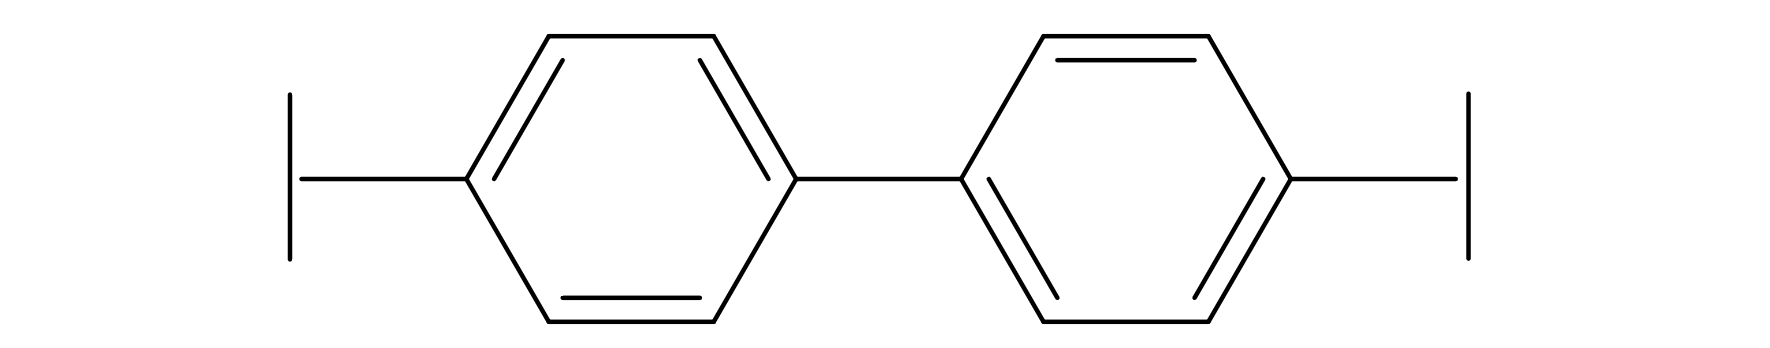
\includegraphics[width=4cm]{structures/DUT-49}
            & Original material & Multiple crystal sizes \\
            \midrule    
        DUT-48  & 
            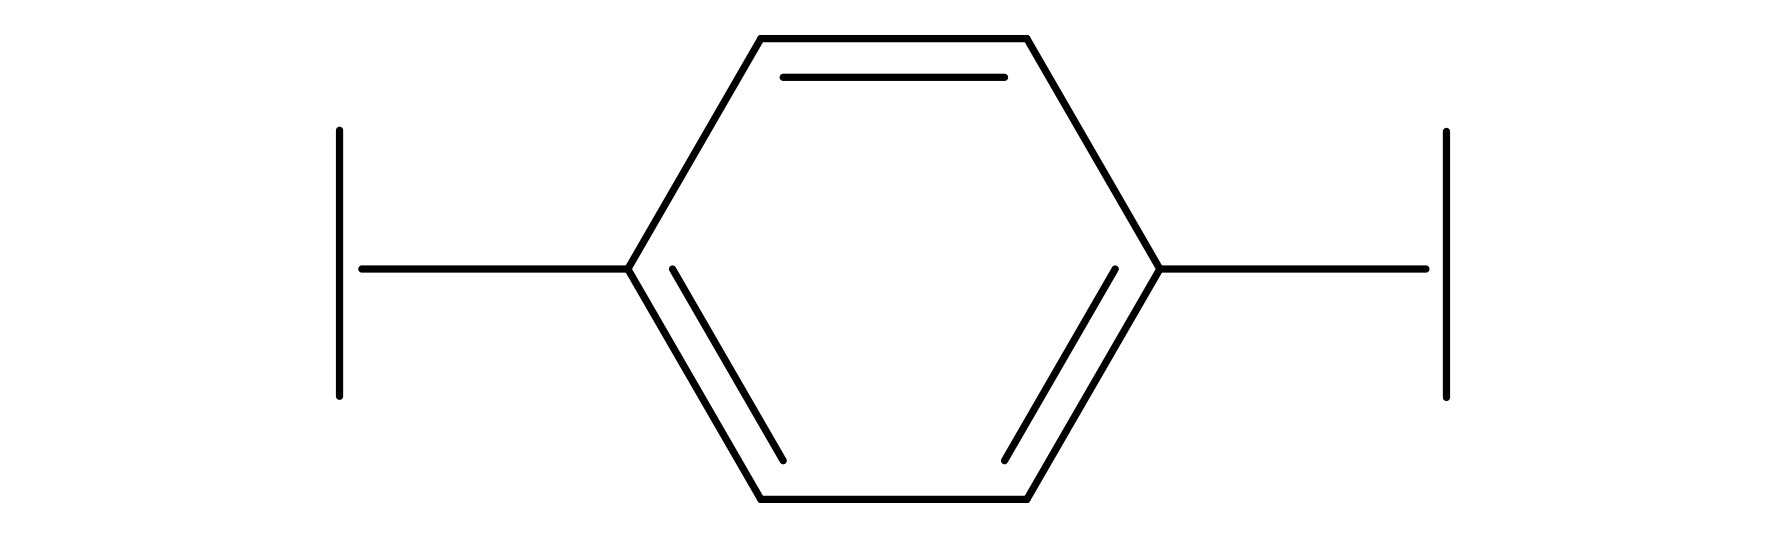
\includegraphics[width=2.5cm]{structures/DUT-48}
            & Linker size & --- \\
        DUT-46  & 
            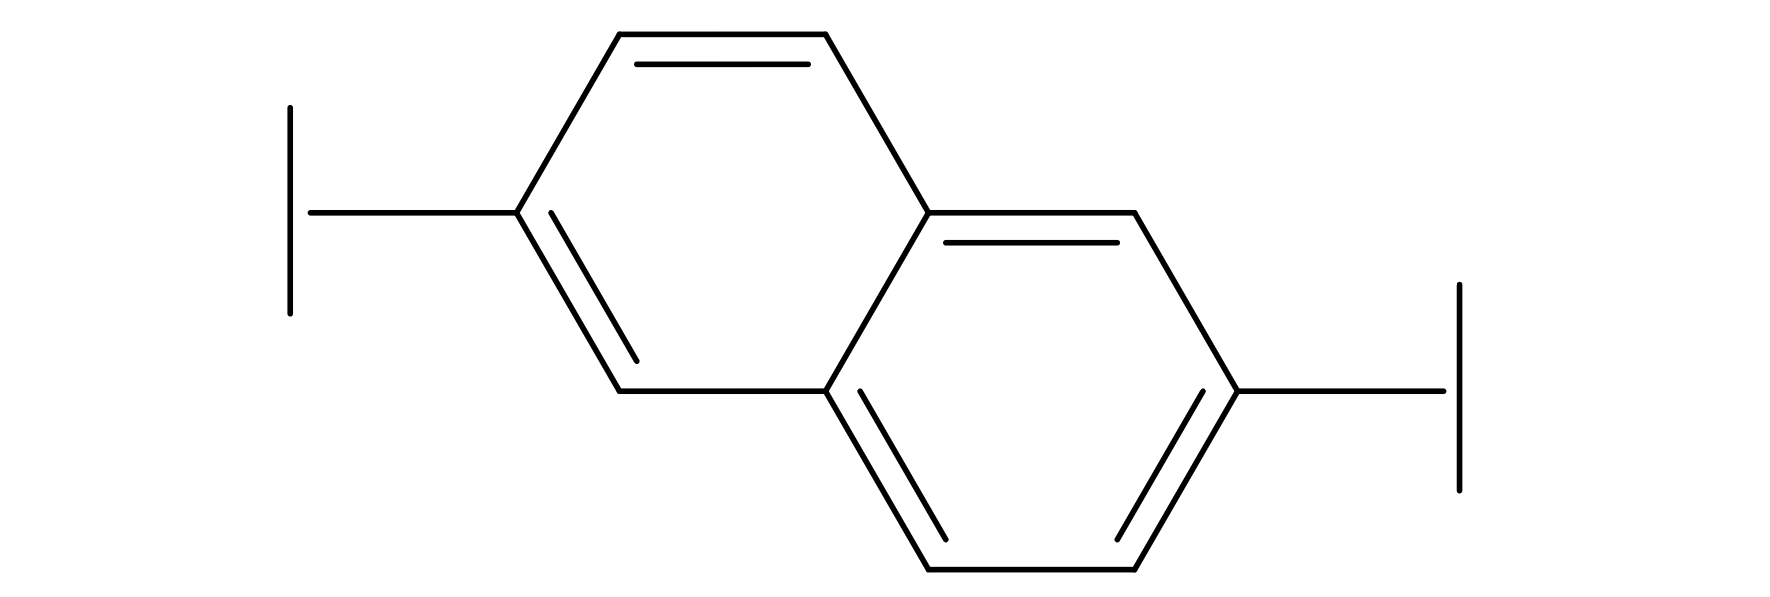
\includegraphics[width=3cm]{structures/DUT-46}
            & Linker size & --- \\
        DUT-50  & 
            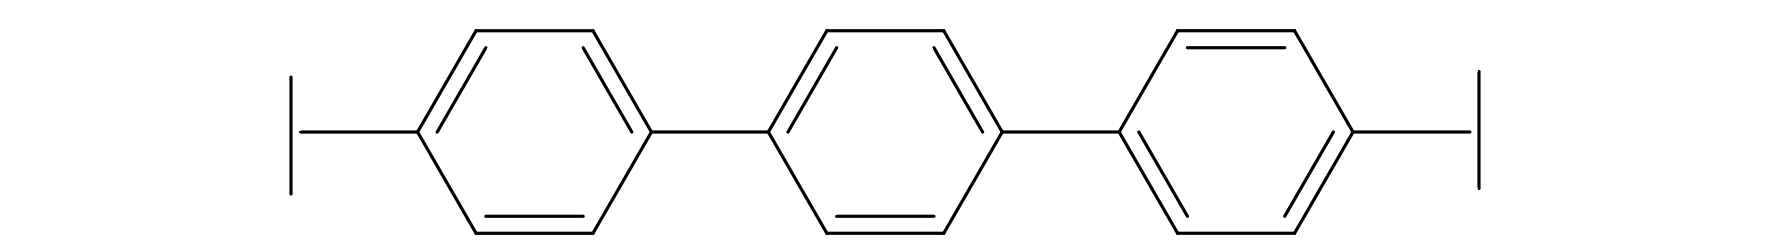
\includegraphics[width=5.3cm]{structures/DUT-50}
            & Linker size & --- \\
        DUT-151  & 
            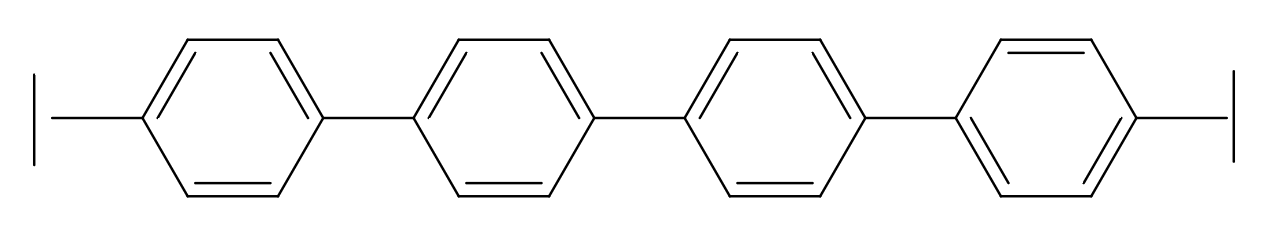
\includegraphics[width=5cm]{structures/DUT-151} 
            & Linker size & Interpenetrated \\
        DUT-152  & 
            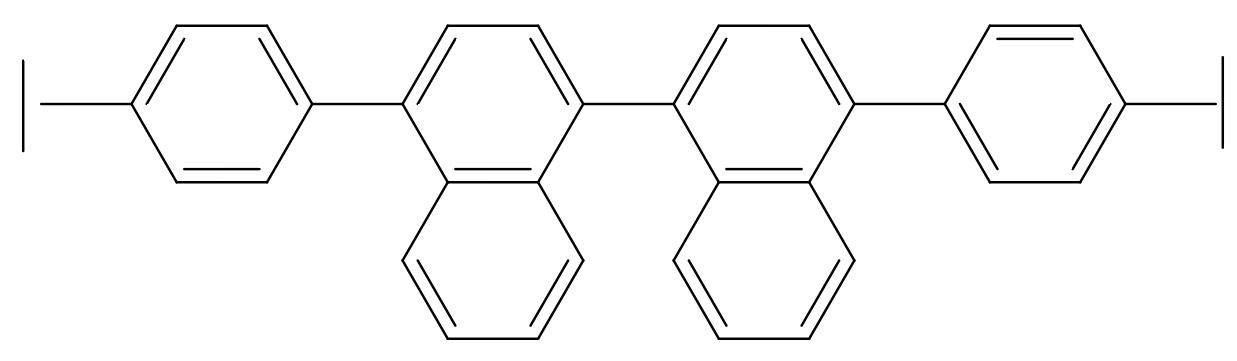
\includegraphics[width=5cm]{structures/DUT-152}
            & Linker size & Interpenetrated \\
            \midrule
        DUT-149  & 
            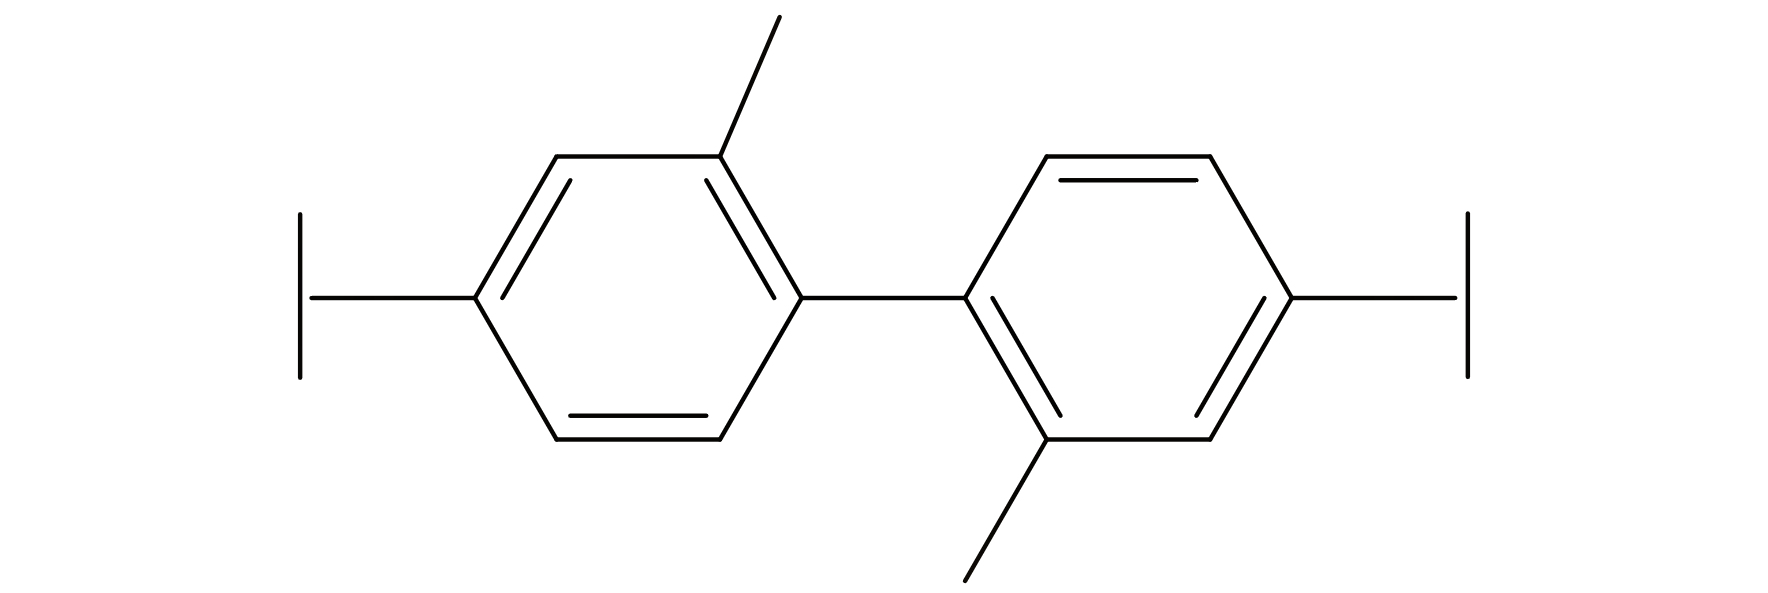
\includegraphics[width=3.8cm]{structures/DUT-149}
            & Functionalization & --- \\
        DUT-148  & 
            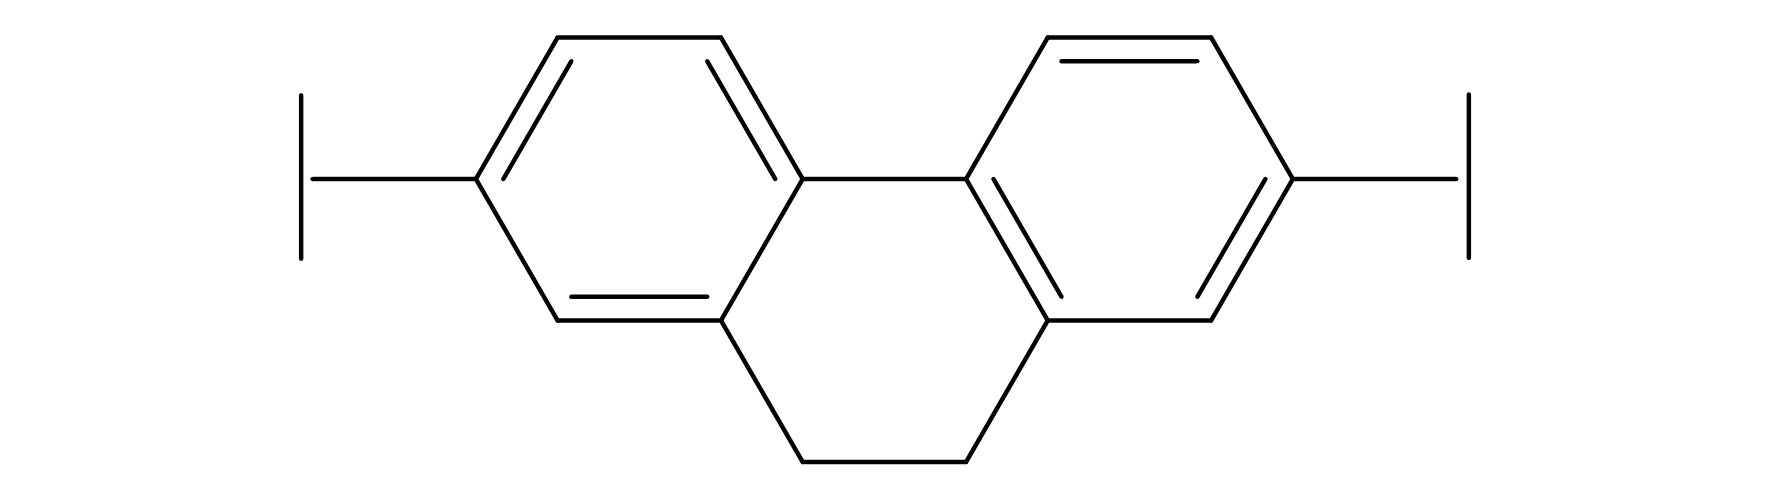
\includegraphics[width=3.8cm]{structures/DUT-148}
            & Functionalization & --- \\
        DUT-147  & 
            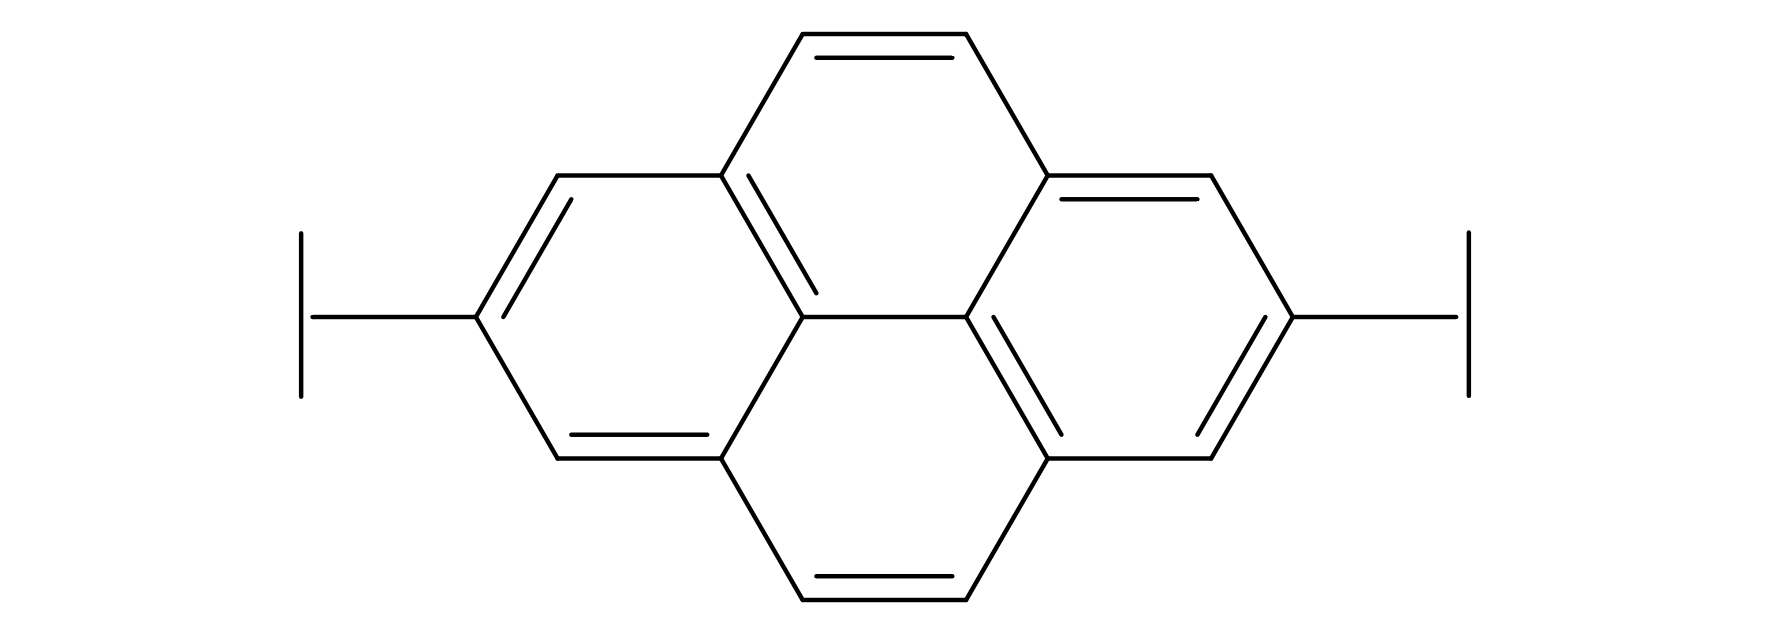
\includegraphics[width=3.8cm]{structures/DUT-147}
            & Functionalization & --- \\
            \midrule
        DUT-160  & 
            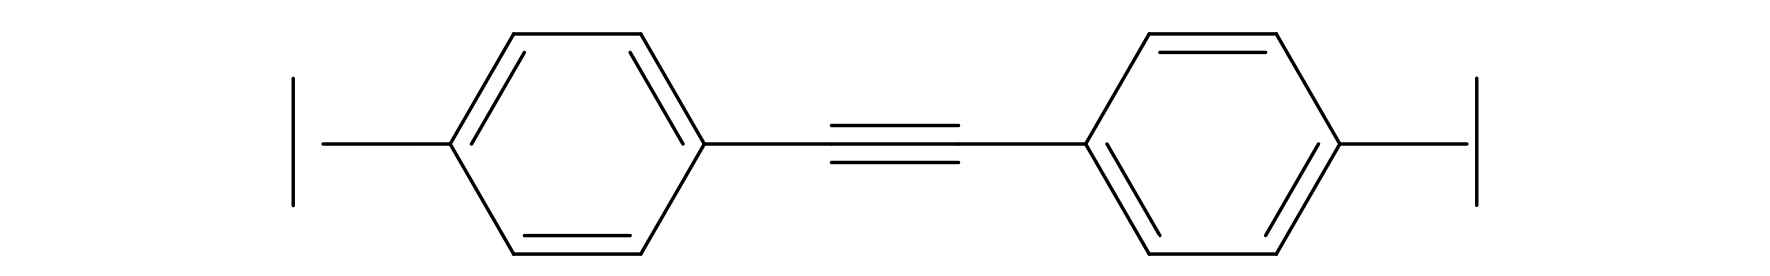
\includegraphics[width=5cm]{structures/DUT-160}
            & Strut saturation & --- \\
        DUT-161  & 
            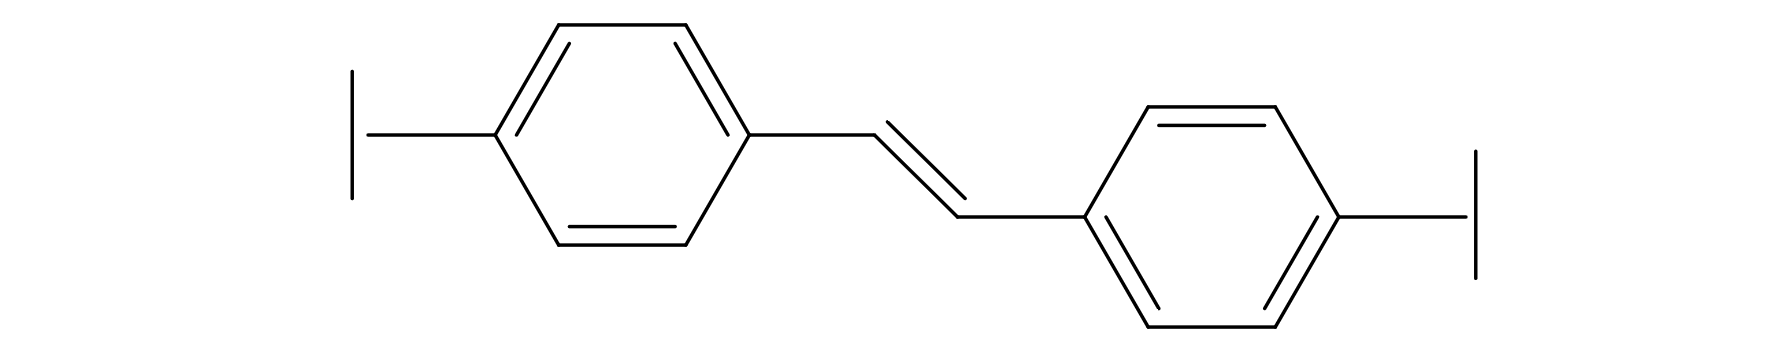
\includegraphics[width=5cm]{structures/DUT-161}
            & Strut saturation & --- \\
        DUT-162  & 
            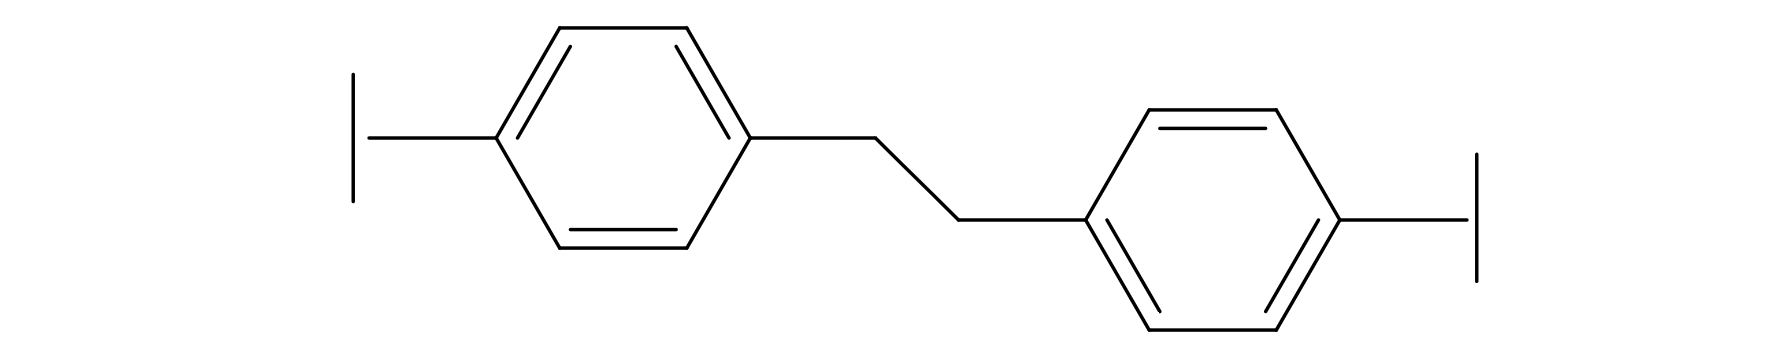
\includegraphics[width=5cm]{structures/DUT-162}
            & Strut saturation & --- \\
            \midrule
        DUT-170  & 
            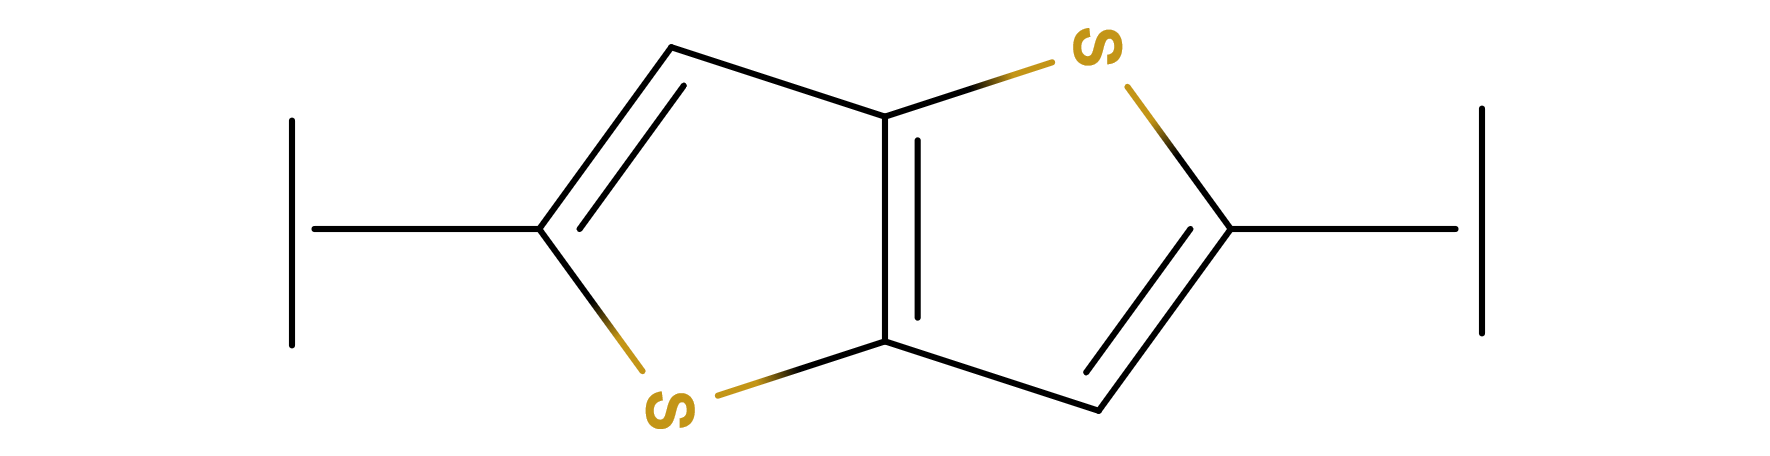
\includegraphics[width=3.2cm]{structures/DUT-170}
            & Heterocycle & --- \\
        DUT-171  & 
            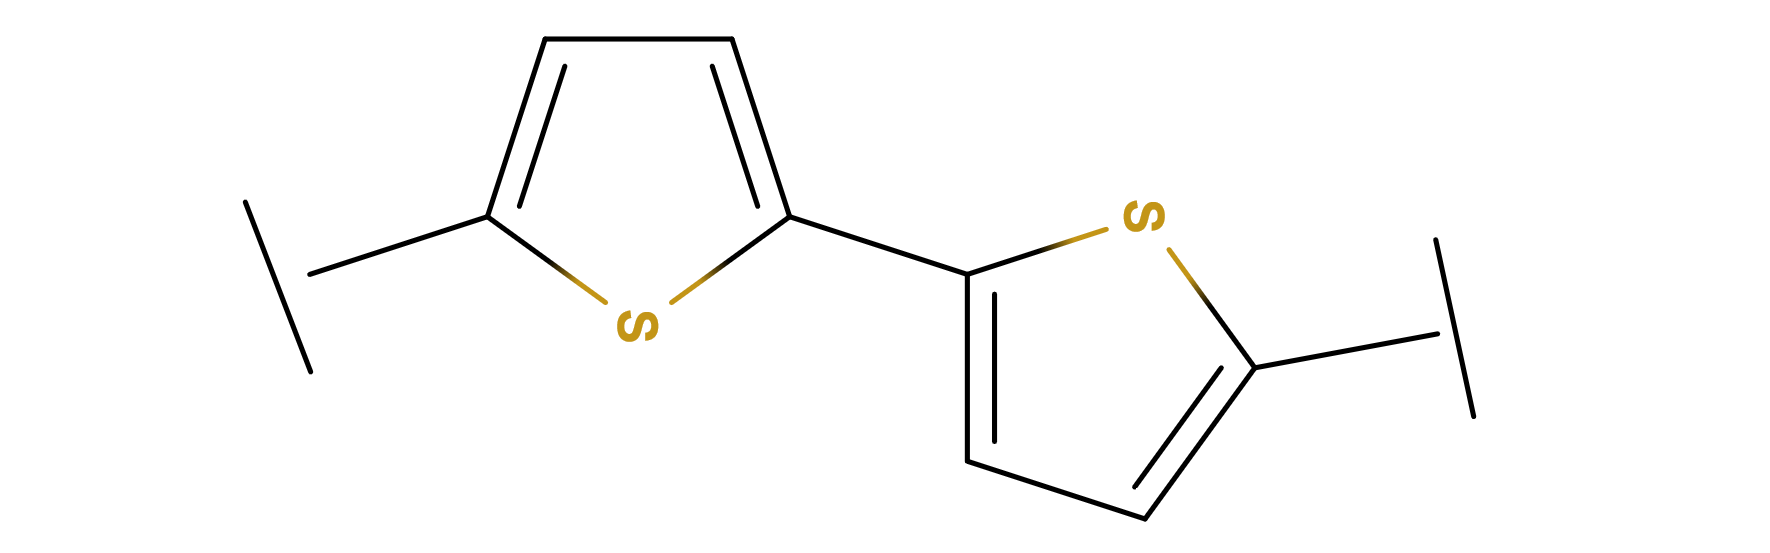
\includegraphics[width=4cm]{structures/DUT-171}
            & Heterocycle & --- \\
        DUT-172  & 
            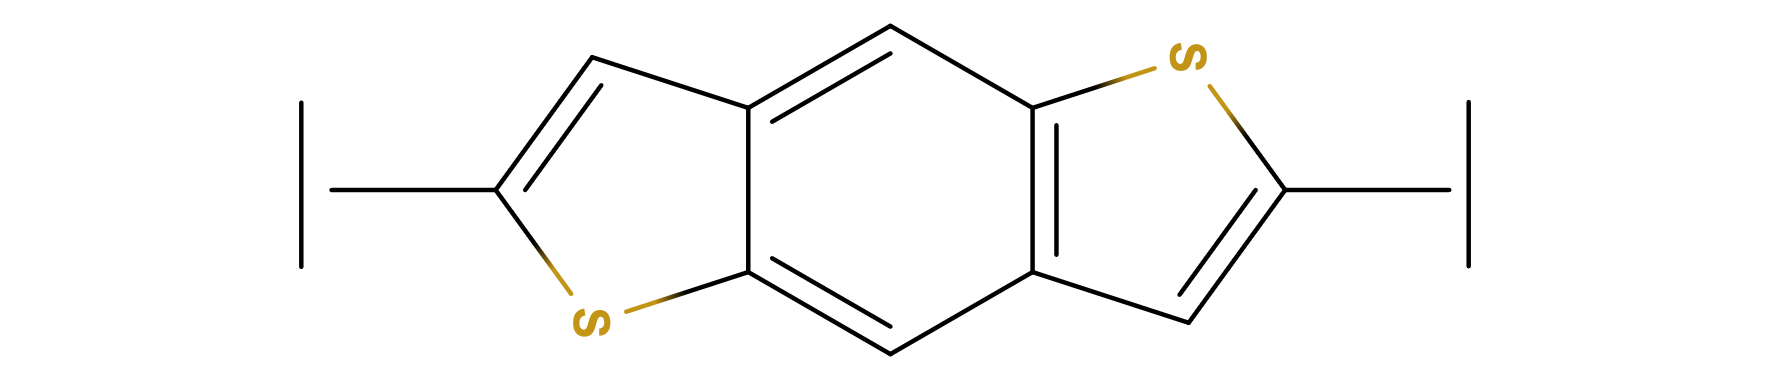
\includegraphics[width=4cm]{structures/DUT-172}
            & Heterocycle & --- \\
        DUT-173  & 
            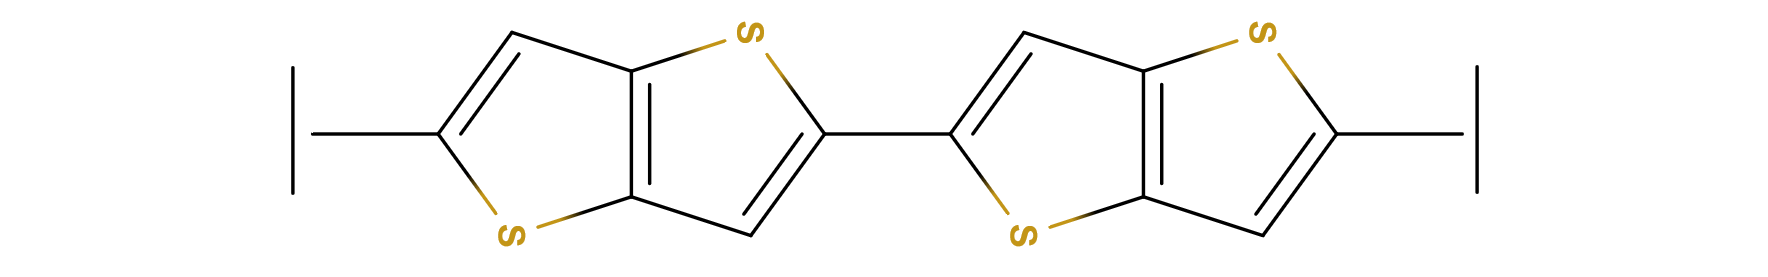
\includegraphics[width=5.5cm]{structures/DUT-173}
            & Heterocycle & --- \\
        \bottomrule
	\end{tabular}%
	\label{dut:tab:materials}
\end{table}%
